\chapter{Reconstruction d'images par interférométrie avec masque irrégulier sur JWST}
%\section{Interférométrie par masque non-régulier}
% Mentionner le scope restreint (Aperture masking, etc.)
% Optical does not mean optical wavelength, only means we are using optics
%to manipulate the light (lens, mirrors,mas)
% Cite Monnier for an excellent review

% History
%La première conceptualisation de l'interférométrie par masque apparaît dans un rapport sur le Concours Bordin de l'année 1867, 


%\blockquote{
        %Il existe en effet pour la plupart des phénomènes d'interférences, tels que les franges d'[Young], celles des miroirs 
        %de Fresnel et celles qui donnent lieu à la scintillation des étoiles d'après Arago, une relation remarquable et 
        %nécessaire entre la dimension des franges et celle de la source lumineuse, en sortes que les franges d'une 
        %ténuité extrêmes ne peuvent prendre naissance que lorsque la source de lumière n'a plus que des dimensions angulaires 
        %presque insensibles; d'où, pour le dire en passant, il est peut-être permis d'espérer qu'en s'appuyant sur ce principe et 
        %en formant par exemple, au moyen de deux franges d'interférences au foyer des grands instruments destinés à observer les étoiles, 
        %il deviendra possible d'obtenir quelques données nouvelles sur les diamètres angulaires de ces astres.
%}

%Pour bien comprendre ce phénomène, on peut utiliser l'expérience des deux fentes de Young. 
%\begin{figure}[H]
        %\centering
        %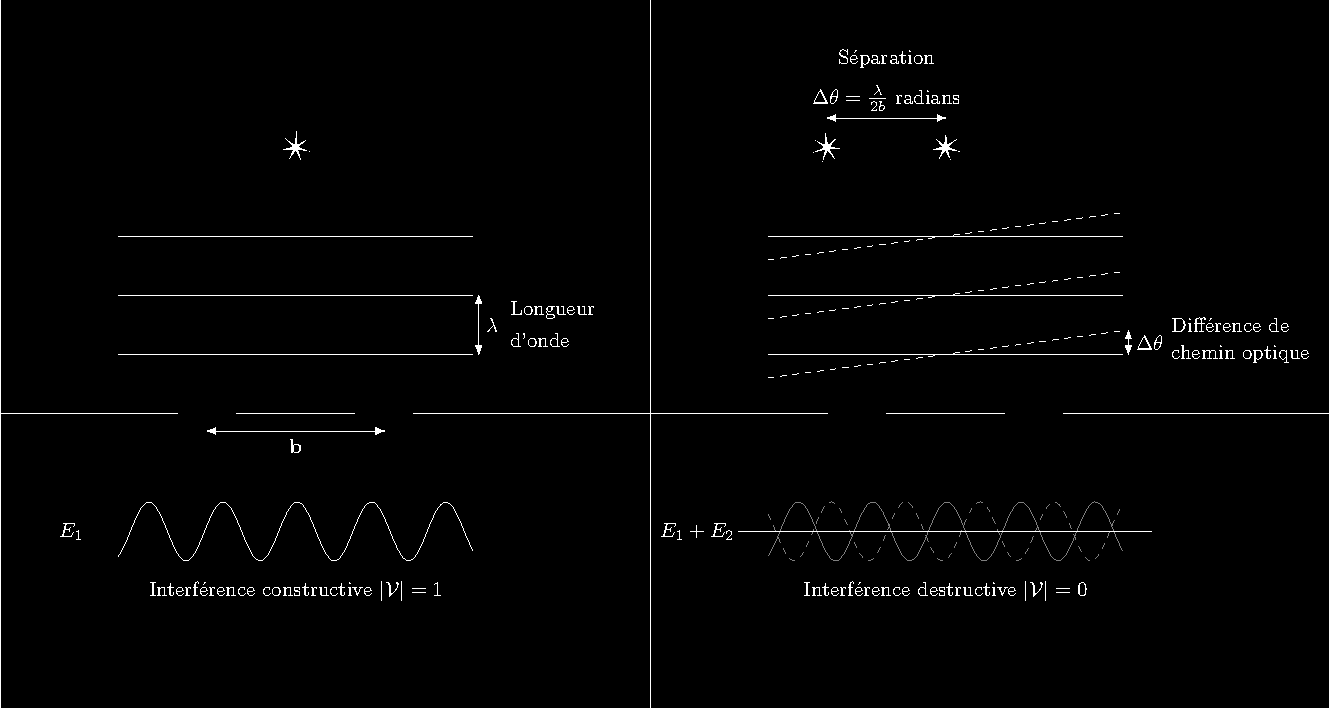
\includegraphics[width=0.8\textwidth]{figures/young_cartoon}
        %\caption{Reproduction de Monnier 2000}
        %\label{fig:young}
%\end{figure}

%Dans le cas où la taille de l'objet est trop petite, le patron d'interférence est celui de gauche. Dans le cas où 
%la taille angulaire, ou la distance angulaire entre deux objets singuliers, atteint un seuil caractéristique 
%$\Delta \theta = \frac{\lambda}{2b}$, nommé le critère de Michelson, alors la visibilité atteint un minimum tel qu'illustré 
%dans le patron de droit dans l'image.
%$\omega = 2 \pi \nu$, $\nu \lambda = c$.
%$D$ est la distance du diamètre angulaire entre la source et les fentes, qu'on prend beaucoup plus grande

%\begin{equation}\label{eq:E1}
        %E_1(\ell, m, t) = A(\ell,m, t - \frac{R_1}{c}) \frac{e^{-i\omega (t - \frac{R_1}{c})}}{R_1} 
%\end{equation} 

%Dans l'approximation où le champ élecromagnétique de deux sources, $E_1$ et $E_2$, sont monochromatique, de longueur d'onde $\lambda$, on 
%peut écrire la luminosité totale observée sur l'écran image comme
%\begin{equation}\label{eq:Itot}
        %\begin{aligned}
                %I(\ell, m) &=  \int_{0}^{T} (E_1(\ell, m, t) + E_2(\ell, m, t)))^{2}dt \\[1.5ex]
                %I(\ell, m) &=  \int_{0}^{T} (E_1(\ell, m, t) + E_2(\ell, m, t)))^{2}dt %\\[1.5ex]
        %\end{aligned}
%\end{equation} 


%%Le truc est donc de changer la longueur de base $\mathbf{b}$ pour obtenir un minimum pour la visibilité
%% Fizeau note 1868 (voir Monnier thesis for source)
%% Michelson applied to measure diameter of Jupyter Moons (1891) and Betelgeuse (1921)
%% Jennison + radio telescopes
%% 90s-20s Optical interferometry with masks
%% Van Cittert-Zernike Theorem 


%% In practice, we go and measure the visibilities and try to take the inverse Fourier transform
%\subsection{Théorème de van Cittert-Zernike}
%Pour obtenir un peu d'intuition sur ce théorème important, on utilise l'expérience classique des deux 
%fentes de \citep{Young}. On considère deux fentes séparées par une distance $\mathbf{D}$, et on illumine ces 
%deux fentes avec de la lumière monochromatique de longueur d'onde $\lambda$.

%% Maybe show picture here
%Supposons

%\begin{equation}\label{eq:Mutual Coherence}
        %\Gamma_{12} = \lim_{T \rightarrow \infty } \frac{1}{2T} \int_{-T}^{T} E_{1}(t)\tilde{E}_2(t - \tau) dt 
%\end{equation} 


%% Time average
%\begin{equation}\label{eq:time average}
        %\langle E_1\tilde{E}_2\rangle_{t} = \langle A(\ell,m,t - \frac{R_1}{c}) \tilde{A}(\ell,m,t - \frac{R_2}{c}) \rangle_t
       %\frac{e^{i\omega(\frac{R_1 - R_2}{c})}}{R_1 R_2} 
%\end{equation} 

%Now $\langle A(\ell,m,t - \frac{R_1}{c}) \tilde{A}(\ell,m,t - \frac{R_2}{c}) \rangle_t = I(\ell, m)$ for incoherent source

%% Explaining the resolution, we need to look at the visibility curve, a binary is resolved when V reaches its minimum (for Michelson interferometry, where we can change the baseline by changing the OPD.

%% Rayleigh Criterion
%\begin{equation}\label{eq:Rayleigh}
       %\Delta \theta_{\text{Télescope}} = 1.22 \frac{\lambda}{D}
%\end{equation} 

%% Micheslon criterion
%\begin{equation}\label{eq:Michelson}
        %\Delta \theta_{\text{Interféromètre}} = \frac{\lambda}{2b} 
%\end{equation} 
%Nearly twice as good.

% Consider two point source (two planar EM waves) 
% Consider two slits, common Young experiment, we get interference fringes. 
% Michelson 1920 defined visibility in term of P_min and P_max 
% See Lawson for the best reference on this

% I could show the little presentation here to showcase Slit experiment and V in term of I_min I_max

% Show a classical Two slit Young experiment
% Generalize this too multiple slits by a simple sum
% Show how to retrieve V from the complex mess (FT)
% From von Citter th, show hyw we try to inverse FT our Vs to retrieve true source emission.

% P = P_0 (1 + Re{V e^ {ik delta}}) (for a single fringe)

% Pupil-plane or Michelson interferometry
% Image plan interferometry <- is what I am doing


%Le théorème de von Cittert-Zernike nous assure que les visibilités mesurées correspondent à la transformée 
%de Fourier de l'intensité de la source, de sortes que le problème de reconstruction d'image par interférométrie et 
%de prendre la transformée de Fourier inverse des visibilitées mesurées.

%Showing what visibilities are, fringes etc.
%Show how fringes emerges, through time averaged cross correlation of EM fields.

%\begin{equation}
        %\tilde{\mathcal{V}}\left( \frac{\mathbf{D}}{\lambda} \right) = \frac{\displaystyle \int_{\Omega}dx_\Omega dy_\Omega I_\lambda (\mathbf{r}_\Omega) e^{-\frac{\mathbf{D}}{\lambda} \cdot \mathbf{r}_\Omega}}{\displaystyle \int_{\Omega} dx_\Omega dy_\Omega I_\lambda (\mathbf{r}_{\Omega})}
%\end{equation}

%En pratique, comme le nombre de mesure n'est pas complet, le problème de reconstruction d'image 
%est mal-posé, et on doit introduire certaine contraintes pour reconstruire les visibilitées qui ne sont 
%pas mesurées. Parler de DFT. 
% montrer un u, v plot

% Solution for binaries, Disk are nice to put here.


% Number of baselines = N choose 2

% Useful citations
%\citep{Sivaramakrishnan2012} Introduction of NIRISS AMI
%\citep{Greenbaum2015} Image plane algorithm for NIRISS AMI
%\citep{Thiebault2017} Review of image reconstruction with optical interferometers
%\citep{Claes2020} Astrophysical prior based image reconstruction (using GAN)
%^\citep{Issaoun2019} VLBI imaging
%\citep{Morningstar2019} Interferometric reocnstruction with RIM
%\citep{Chael2018} ELT direct optimisation of bispectra
% \citep{Pope2016} Kernel phase and kernel amplitude in Fizeau imaging
% \citep{Fizeau1868} Aperture masking 
% \citep{Jennison} Closure phases
% \citep{Monnier1999} Phd thesis, aperture masking with Keck to analyze circumstellar disks
% \citep{Monnier2007} Review
% \citep{Tuthill1999} Surface imaging of a variable star

%\subsection{Les angles de fermeture}

